\chapter{Interpreting calculation results}\label{ch:results}

After a calculation, use its figures, data, and workflow together to interpret the results. Figures reveal trends, data records establish their origin, and the saved workflow specifies the calculation conditions. This chapter explains how to read these materials and turn them into conclusions you can support in a report or research notebook.

The hydrogen molecule and silicon examples illustrate single-point energies, atomic forces, geometry optimization, band structures, and densities of states. For your own results, ask three questions in order: Did the calculation finish? How is the plotted quantity defined? What conclusion can it support?

\section{Find results in the project}

\subsection{Where results are stored}

Open the \ui{Project Browser} from the left sidebar and expand \ui{Results}. \ui{Datasets} holds datasets; \ui{Plots} holds figures. A dataset records information from a run, while a figure presents part of it in a readable form. Band, DOS, and convergence plots are all graphical results, but represent different quantities.

Double-click a figure generated by the current version to reopen it. If its document is already open, the application activates it. Figure objects from older projects may not survive a version change; the procedures below redraw them from saved numerical data. Before comparing runs, identify the figure and its associated run record. A result retained in a project does not automatically update when you edit a node.

For example, changing Ecut from $20$ to $30$ Ha leaves the existing convergence plot associated with the $20$ Ha run. Run the workflow again to generate results for the new cutoff. Give each trial figure a descriptive name promptly rather than accumulating indistinguishable defaults.

\subsection{Read the record before the figure}

A figure can expose a problem quickly, but can also conceal inconsistent conditions. Check the structure, functional, pseudopotentials, cutoff, and sampling first, especially when a project contains several structures. For optimization, distinguish initial and final geometries.

A report need not reproduce the log line by line, but retain the original record. State key conditions in captions and keep complete inputs in an appendix or accompanying files. This keeps the text readable while allowing important numbers to be checked.

\section{Read a dataset}\label{sec:read-dataset}

Select a run under \ui{Results → Datasets} and check its name, time, and description in the Information Browser. Labels usually begin with \ui{Run}, followed by the workflow name used at execution. Distinguish similar records by their input conditions, not just their order in the list. The current Information Browser does not expand all numerical values in these calculation datasets; inspect the underlying contents in full MATLAB\regmark{} or the appropriate command workspace.

The table below identifies common names encountered after exporting a dataset, linking each array to its producing task. The next section explains how to export a selected dataset to the workspace.

\begin{table}[htbp]
\centering
\caption{Common result-data names.}
\begin{tabularx}{\linewidth}{lX}
\toprule
Name & What to check first \\
\midrule
info & SCF status, total energy, and energy/error histories; after optimization, it may describe the last ionic step. \\
relaxInfo & Geometry optimization history; distinguish it from the initial structure's single-point info. \\
symmetry & Primitive-cell and high-symmetry-path information for checking the band calculation. \\
bandProcessing & Path $k$ points and band arrays; interpret the horizontal axis using that path. \\
bandProcessing3D & $k$ points, energies, and plane names for reciprocal-space planes. \\
DOS & Energy samples and total density of states, rather than an atom-projected DOS. \\
TDDFT & Excitation energies Et and transition vectors Z; check completion and energy units first. \\
\bottomrule
\end{tabularx}
\end{table}

Not every run contains all these entries. SCF alone does not produce DOS, and symmetry analysis alone does not produce electronic energies. Electronic states and other data may also be stored as objects whose full details are not expanded in the Information Browser. Use figures and logs for routine inspection, and full MATLAB\regmark{} or the supplied scripts for further array processing.

Geometry optimization results are stored in the run record, while the Structure branch retains the original model. To inspect the final geometry in 3D, import the optimized structure file as in the hydrogen example and compare it with the optimization record.

\subsection{Export a selected project item to the workspace}

\ui{Home → Variable → Export variable to MATLAB workspace} exports the selected Project Browser item to the corresponding workspace. It transfers the project-item object rather than generating a CSV table; save files separately according to their intended use. The variable name is derived from the item's display name, with spaces removed and invalid variable-name characters adjusted.

\begin{steps}
\item In the toolbox running in full MATLAB\regmark{}, select the required dataset and give it an easily recognized display name, such as \texttt{H2Run}.
\item Choose \ui{Home → Variable → Export variable to MATLAB workspace}.
\item In MATLAB\regmark{}'s own Command Window, use \texttt{whos} to check the variable, read its \texttt{data}, and inspect the available data names.
\item Check units, structure, and dimensions before reading arrays. Save a MAT file or results table as needed, and retain the original project.
\end{steps}

Online places the selected object in the application's command workspace, which differs from full MATLAB\regmark{}'s base workspace. Standalone users can inspect figures directly and retain results by saving projects and exporting images.

The following illustrates reading an already exported SCF dataset in full MATLAB\regmark{}. Use the variable name actually created by your export.

\begin{lstlisting}[language=Matlab]
runData = H2Run.data;
keys(runData)
scfInfo = runData('info');
scfInfo.Etot
scfInfo.converge
save('h2-run-data.mat', 'runData');
\end{lstlisting}

For a figure, structure, or record from another workflow type, inspect its data names before choosing fields.

\section{Check electronic convergence}
\index{Convergence checks}

\subsection{The status is more direct than the curve's appearance}

The convergence message at the end of an SCF log states whether the solver met its criteria. A flattening energy curve is useful evidence but cannot replace that check. Small unconverged changes can be almost invisible against a large negative total energy.

The hydrogen reference run finishes with a relative density error of approximately $8.85\times10^{-9}$; the eight-atom silicon cell finishes at approximately $7.35\times10^{-9}$. Both meet their specified electronic criteria. Your intermediate iterations need not match every point, but the final status should meet the intended conditions.

\subsection{Read a convergence plot with two vertical axes}

The horizontal axis counts electronic iterations. The blue energy curve uses the left Energy (Ha) axis; the orange error curve uses the right Error axis. Their units and scales differ, so their intersections have no physical significance.

The error axis is logarithmic. A decrease from $10^{-3}$ to $10^{-6}$ is three orders of magnitude, not three units. Look first at the overall trend, then at any repeated oscillations, and finally at whether the stopping criterion was met.

In the hydrogen example, the energy approaches its final value before the density finishes converging. Different indicators need not stabilize together. For forces or small energy differences, use sufficiently strict electronic accuracy rather than stopping manually when the energy curve looks smooth.

\subsection{Three common convergence patterns}

If the error keeps decreasing but reaches the iteration limit, more iterations may allow that trend to finish. If it oscillates between two or more levels, check the structure, occupations, and numerical settings. Nonfinite values or clearly abnormal energies from the outset call for checking atomic separations, the cell, and pseudopotential loading.

These patterns require different responses. A complete stretch of iteration history is more informative than ``the run failed.'' Comparing with a small successful example also helps distinguish a new-system problem from an environment-wide issue.

\section{Compare total energies}
\index{Total energy}

\subsection{Identify the system an energy belongs to}

Total energy depends on the elements and atom count, geometry, functional, pseudopotentials, and numerical conditions. Absolute energies of different systems generally cannot be ranked directly. The eight-atom silicon cell having a more negative energy than a hydrogen molecule does not establish that silicon is more stable: the two numbers describe different atomic and electronic systems.

For cells with the same composition but different sizes, normalize per atom or formula unit. Adsorption, reaction, and defect studies require energy differences constructed from the relevant reaction and reference states. Define the comparison before subtracting energies.

\subsection{Practice with the hydrogen molecule}

With the same box, functional, pseudopotentials, and cutoff, the initial hydrogen geometry has total energy approximately $-1.1652136531$ Ha; the optimized geometry has approximately $-1.1659737582$ Ha. The lower value shows that the optimizer found a lower-energy geometry within this model.

The difference is approximately $-7.60\times10^{-4}$ Ha. It is the energy change from this starting geometry to the optimized structure, not the binding energy relative to two isolated hydrogen atoms. Binding energy requires suitable atomic reference states; an optimization's energy decrease is not a reaction energy.

Tabulate the structure name, bond length, total energy, final force, and convergence status. Such a table relates geometry to electronic results and explains more than an energy column alone.

\begin{table}[htbp]
\centering
\caption{Results from the hydrogen molecule reference run.}
\begin{tabularx}{\linewidth}{lX}
\toprule
Quantity & Reference value\\
\midrule
Initial bond length & $1.50000000$ Bohr, approximately $0.79376582$ Å\\
Initial total energy & $-1.1652136531$ Ha\\
Optimized bond length & $1.43107436$ Bohr, approximately $0.75729194$ Å\\
Optimized total energy & $-1.1659737582$ Ha\\
Final force norm & Approximately $5.55\times10^{-5}$ atomic units\\
Conditions & PBE, built-in default pseudopotentials, 20 Ha, a 10 Bohr cubic box\\
\bottomrule
\end{tabularx}
\end{table}

Report an appropriate number of digits. Many decimal places do not confer physical accuracy when the model and numerical inputs have not been thoroughly converged. These reference values help check the supplied example.

\section{Check the optimized structure}
\index{Atomic forces}

\subsection{Forces and equilibrium positions}

Atomic forces describe how energy changes with atomic positions. Moving in an appropriate direction along a force generally lowers the energy. For hydrogen, the bond-direction forces are easiest to inspect, and the symmetric arrangement normally gives corresponding forces on the two atoms.

A lower energy does not automatically mean that every atom is at equilibrium. Check the final forces and the optimizer's stopping reason. Reaching the step limit may leave optimization unfinished; sufficiently small forces provide stronger evidence for an equilibrium geometry within the chosen model.

\subsection{Inspect the final geometry}

Open the optimized structure and first check that the elements and atom count are unchanged. Then measure the relevant bond lengths, angles, or lattice parameters. Overall translation and rotation do not change a molecule's internal geometry. Compare relative positions rather than whether an individual atom's absolute coordinates changed.

The Geometry Optimization tutorial relaxes atomic positions in a fixed cell. To study a lattice constant, choose an appropriate scheme explicitly, such as comparing energies at several fixed lattice parameters with consistent treatment of internal coordinates.

\subsection{What a local minimum means}

An optimizer starts from the supplied geometry and searches nearby for lower energy. This is straightforward for a diatomic molecule, but a complex molecule, adsorbate, or defect may have several locally stable configurations. One successful optimization does not exhaust every possible structure.

Optimize from several physically meaningful starting configurations and compare their final geometries and energies. Name each starting point clearly and keep its provenance, so that a selected lower-energy structure remains traceable.

\section{Read a band structure}
\index{Band structures}

\subsection{Open the supplied project's bands}

\file{silicon-band-primitive.ks} contains a two-atom silicon primitive cell, a band workflow, and reference numerical records. If an older figure reports a deleted object, redraw the saved band and DOS arrays using \file{show_reference_results.m}.

This procedure uses the toolbox interface in full MATLAB\regmark{} and does not repeat the DFT calculation. In the standalone or Online edition, run the corresponding workflow from Chapter~\ref{ch:workflows} to generate a current-version figure.

\begin{steps}
\item Start the toolbox in full MATLAB\regmark{} and open \file{silicon-band-primitive.ks} through \ui{Home → Open}. Check its two-site Si structure under \ui{Structure} and keep this project active.
\item Set MATLAB\regmark{}'s current folder to this manual repository's root, then run the following in MATLAB\regmark{}'s own Command Window:
\begin{lstlisting}[language=Matlab]
addpath(fullfile(pwd, 'docs', 'manual-zh-CN', 'examples'));
show_reference_results("bands");
\end{lstlisting}
\item Wait for the \ui{EnergyBandStructure} document and its new \ui{Results → Plots} entry. Match it to the \ui{Energy Band} workflow and confirm the two-atom primitive-cell reference with 8 points per segment.
\item Read the high-symmetry labels and energy units, then use the axes tools to inspect the region near zero. Restore the full view afterward rather than examining only an enlarged fragment.
\item Export the figure and save the project as your own copy. If an old figure becomes unavailable later, redraw the saved numbers instead of rerunning the electronic solver merely to recover an image.
\end{steps}

Figures~\ref{fig:si-band-results} and \ref{fig:si-bands-native} use the same primitive-cell reference data, path coordinates, and energy zero. The figure document supports zooming and interactive inspection.

\begin{figure}[!htb]
\centering
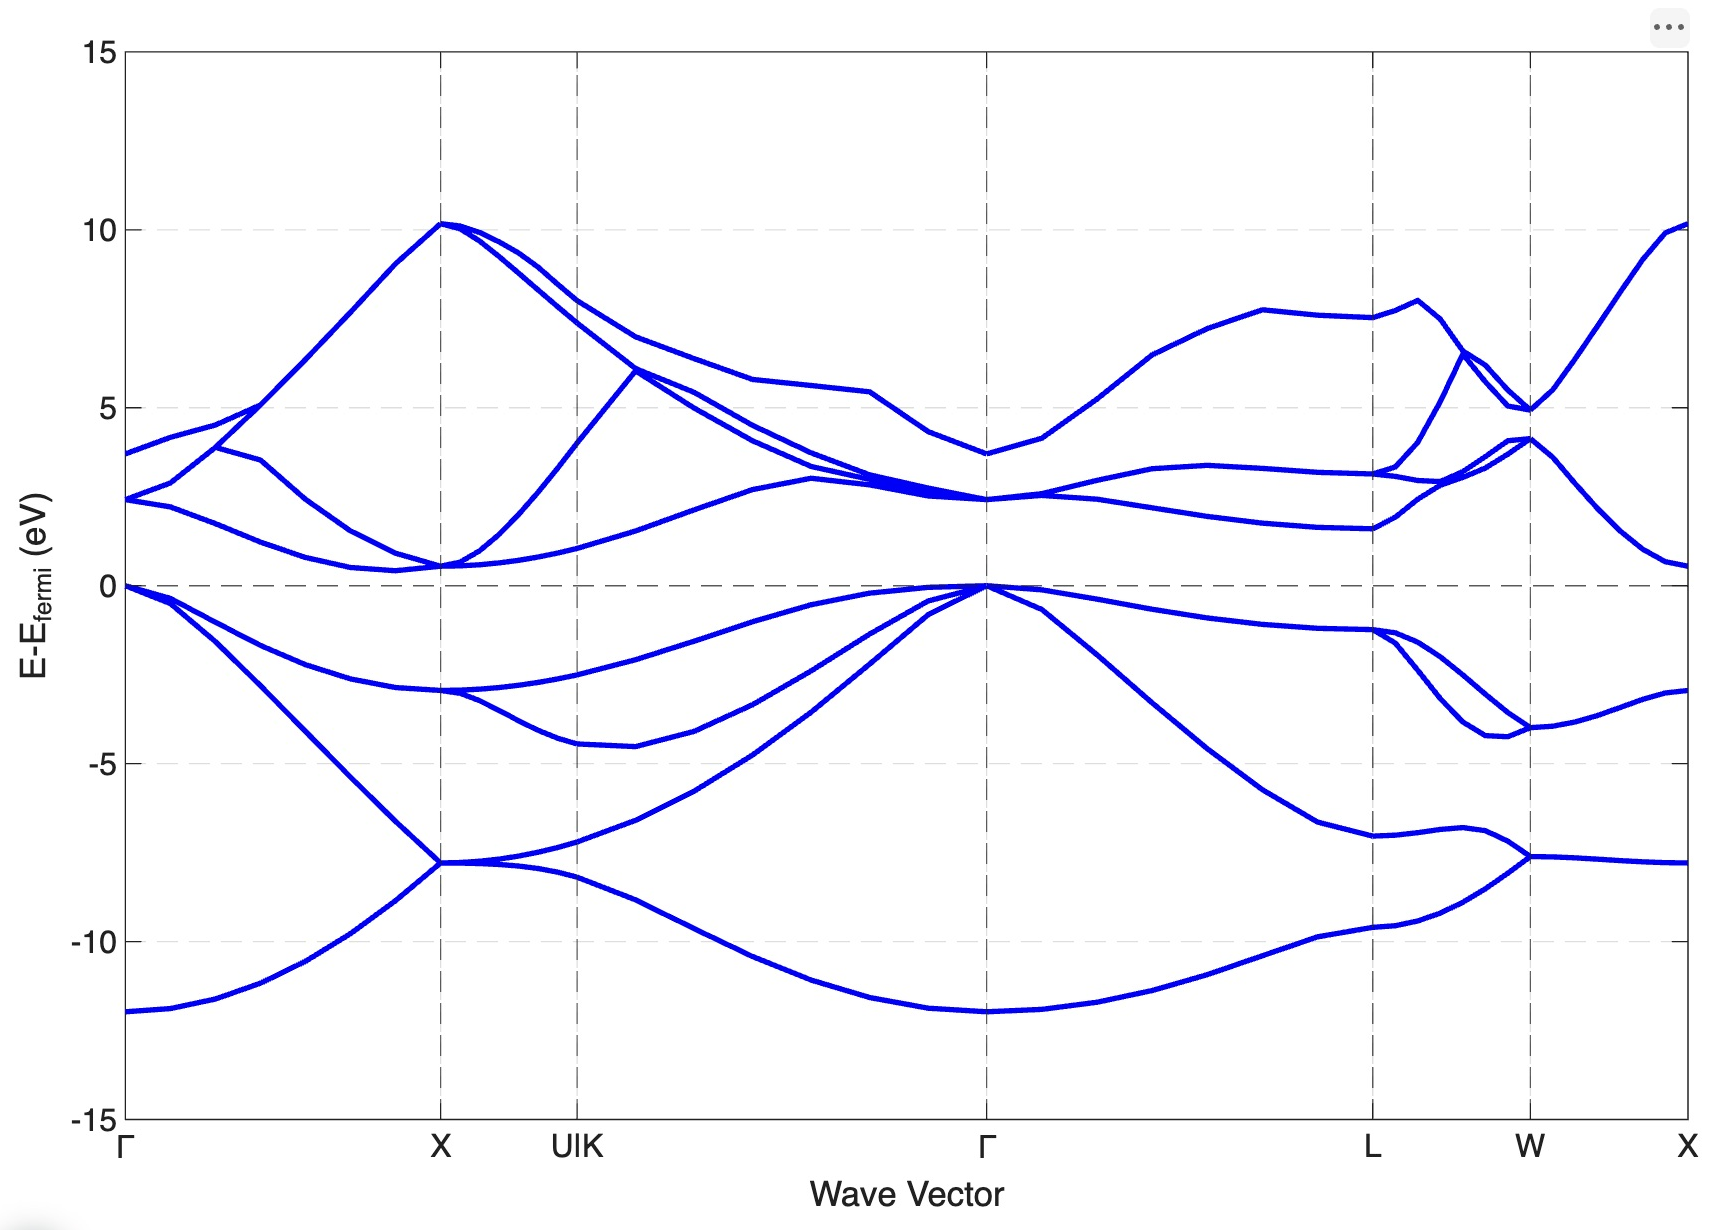
\includegraphics[width=\linewidth]{publication-assets/revision-silicon-bands-live.png}
\caption{The two-atom silicon primitive-cell band document, with 8 points per path segment and the Fermi energy set to zero.}
\label{fig:si-bands-native}
\end{figure}

\subsection{Check the axes and energy reference}

The horizontal axis follows a path through high-symmetry points; the vertical axis is energy. Here it shows $E-E_{\mathrm{fermi}}$ in eV, so zero is the calculated Fermi-energy reference. Separators and labels distinguish path segments, which need not all join continuously in reciprocal space.

Horizontal positions follow distance along the path rather than any single $k$ coordinate. Identify the path labels, inspect occupied and unoccupied states near the Fermi energy, and then examine deeper valence or higher unoccupied states.

Each curve is a band branch, not an atomic trajectory. This example stores eight bands, all drawn in blue; the color does not encode an element, orbital, or spin. Reading along one curve follows its energy along the path. Reading vertically at one horizontal position compares different bands at the same $k$ point.

Vertical dashed lines mark segment boundaries. Disconnected segments can have combined labels: \ui{U|K} means the preceding segment ends at U and the next starts at K, not that there is a new point named U|K. Do not interpret the curves across that boundary as continuing along a single reciprocal-space direction.

\subsection{Identify a band gap}
\index{Band gaps}

In the usual semiconductor picture, the highest occupied bands are valence bands and the lowest unoccupied bands are conduction bands. Their edge-to-edge energy difference is the band gap. A gap is direct when both extrema occur at the same $k$ point and indirect when they occur at different points.

A finite path need not pass through the true band extrema. A smooth plot alone cannot establish the Brillouin-zone minimum merely because no lower conduction state appears on the chosen path. Quantitative gap studies require adequate sampling and band-edge analysis.

The silicon tutorial uses a coarse introductory grid to make the workflow and plotting procedure accessible. State those conditions before discussing how sampling and the functional may affect a quantitative gap.

\subsection{Compare band plots}

Check the cell, path, energy zero, functional, pseudopotentials, and number of bands. Switching between primitive cells and supercells can fold bands; additional curves need not indicate new physical states. Changing the energy reference can shift an entire plot vertically.

For a strain study, use a consistent calculation procedure, converge each structure self-consistently, and choose comparable paths. Identify the bands and $k$ points where changes occur before refining the sampling. Rule out inconsistent numerical conditions before interpreting every small shift as a physical effect.

\section{Read the total density of states}
\index{Density of states (DOS)}

\subsection{Open and check the total DOS}

Continue with \file{silicon-band-primitive.ks}. This two-atom project also stores total DOS values on a $4\times4\times4$ grid. Redraw them without closing the project or running a new DOS workflow.

\begin{steps}
\item Confirm that the two-atom primitive-cell project is active. In the MATLAB\regmark{} Command Window, with the example directory already on the path, run:
\begin{lstlisting}[language=Matlab]
show_reference_results("dos");
\end{lstlisting}
\item Wait for \ui{Density of States (DOS)} and check its new \ui{Results → Plots} entry. This figure is the current Si2 primitive-cell result, distinct from the separate eight-atom project.
\item Read the vertical \ui{Energy (eV)} axis first, then the horizontal \ui{Density of States (DOS)} axis. A curve extending farther right indicates more states near that energy. Do not read energy from left to right as in a conventional energy-on-horizontal-axis plot.
\item Locate zero on the vertical axis and inspect the regions below, near, and above it. Describe populated intervals, low-DOS regions, and main peaks before focusing on small variations.
\item Export the curve using the figure's save tools and retain the project with its original data. Reopen the image to check that both axes are included.
\end{steps}

The data samples $-10$ to $10$ eV in $0.05$ eV steps, using PBE, default pseudopotentials, and a 20 Ha cutoff. To change the grid or energy range, import the \ui{DOS} template as in Chapter~\ref{ch:workflows}, select the two-atom cell, and run with new parameters. Redrawing existing arrays does not improve their sampling accuracy.

\begin{figure}[!htb]
\centering
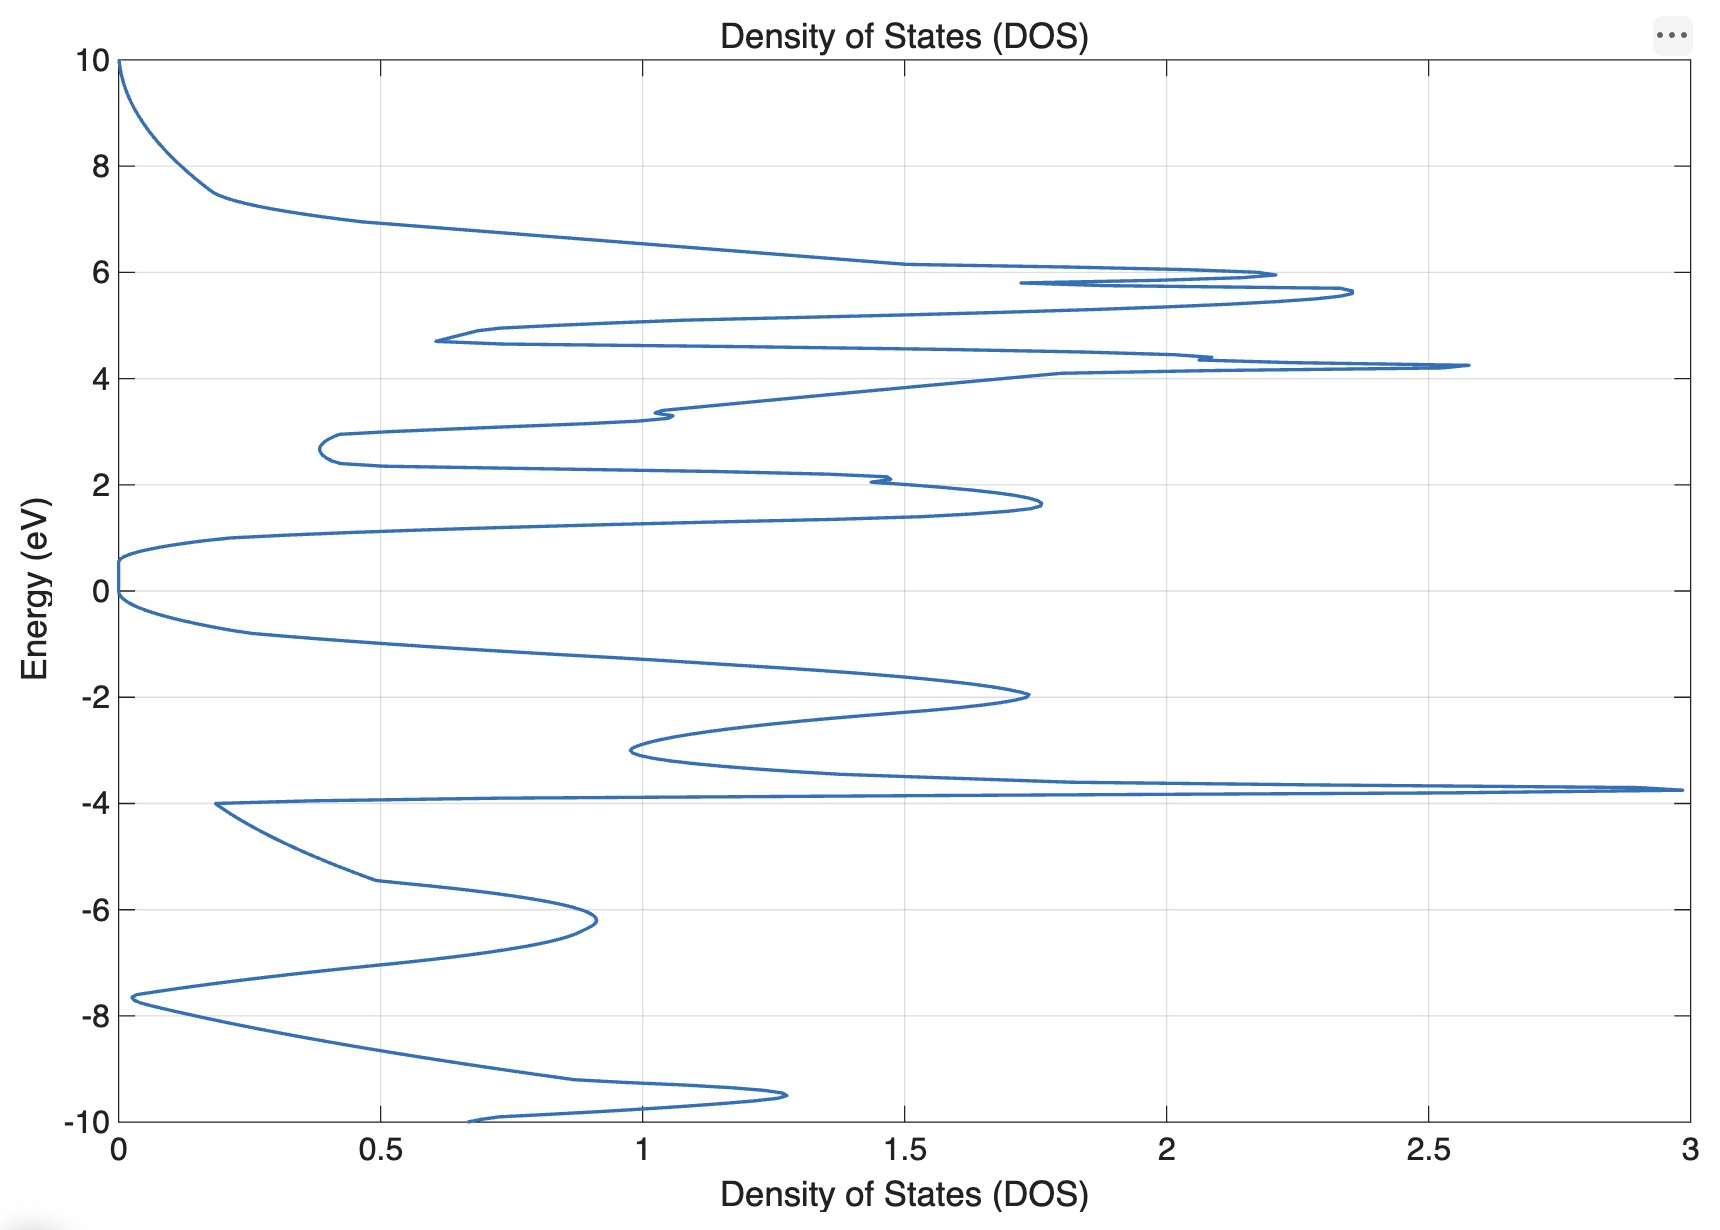
\includegraphics[width=\linewidth]{publication-assets/revision-silicon-dos-live.png}
\caption{Total DOS of the same two-atom silicon primitive cell. DOS is horizontal; energy relative to the Fermi energy is vertical.}
\label{fig:si-dos-native}
\end{figure}

\subsection{Peaks and low-density regions}

A high DOS means that many electronic states lie near that energy. Peaks often reflect band dispersion, but do not identify which atoms or orbitals contribute. That requires projection or composition analysis.

The DOS node gives the total density of states, combining orbitals and $k$ points. Element- or orbital-resolved assignments require the corresponding projected DOS data.

\subsection{Read bands and DOS together}

With a common energy reference, locate the Fermi energy and identify intervals with many states or no states. Bands show variation along a path; DOS summarizes sampling over a grid. They describe the electronic structure from complementary perspectives.

\file{silicon-tutorial.ks} stores DOS for an eight-atom conventional cell. Opening that project and running the same \texttt{show\_reference\_results("dos")} command redraws the Si8 result. Figure~\ref{fig:si-dos-results} retains that eight-atom reference for reading axes and peak shapes. It uses a different cell from the primitive-cell figure above. Normalize consistently per cell or per atom and align conditions and energy references before comparing them.

\begin{figure}[!htb]
\centering
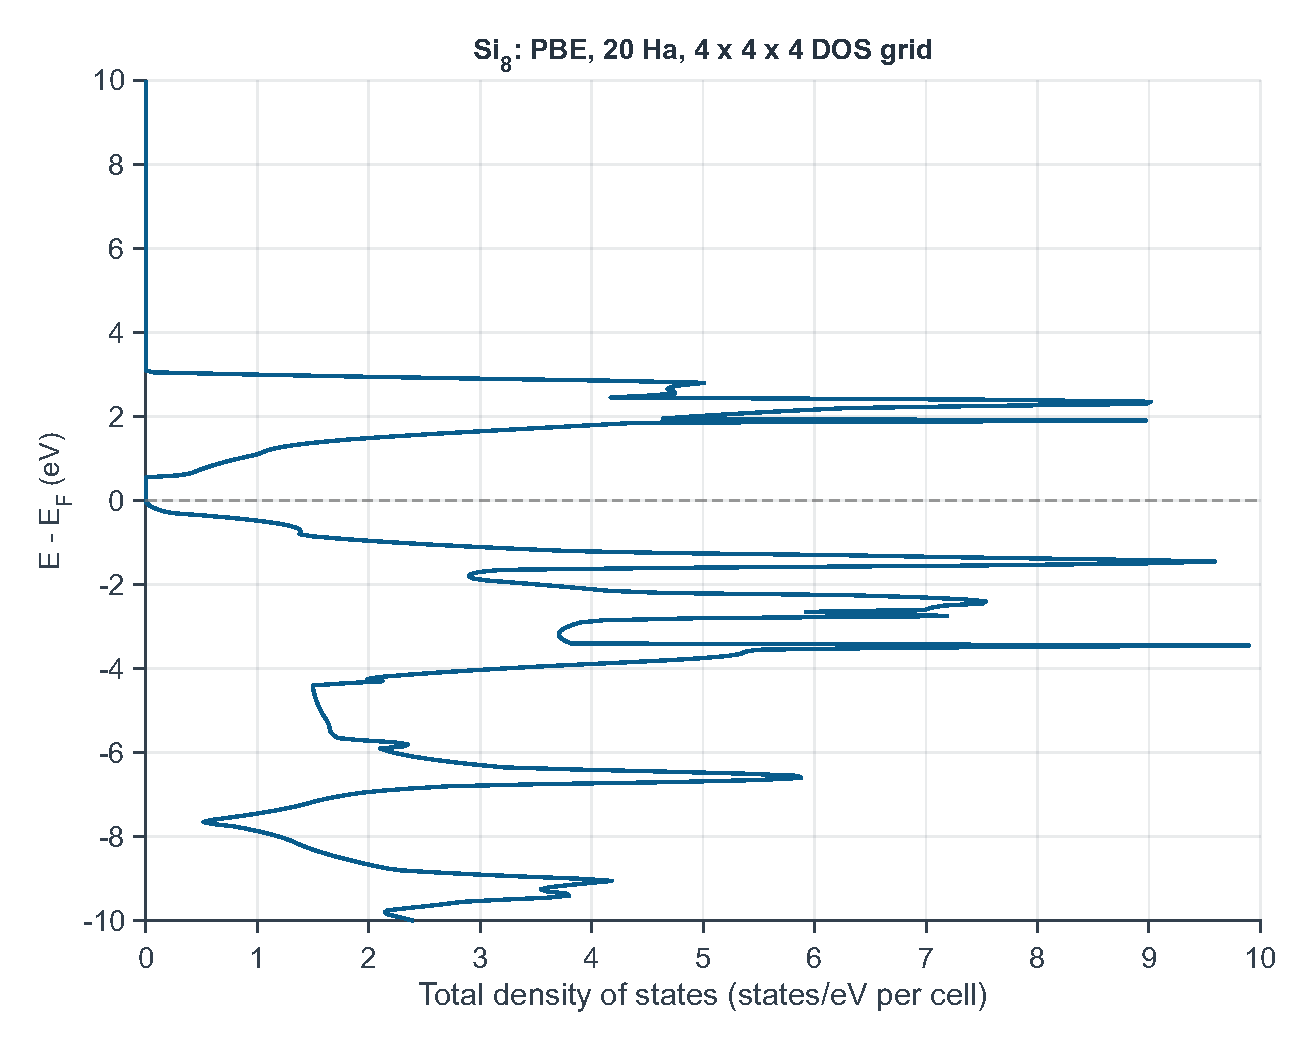
\includegraphics[width=\linewidth]{publication-assets/vector-02b7a0240bc7f99a0fc6.pdf}
\caption{Reference total DOS for the eight-atom silicon cell. The horizontal axis counts states per cell per eV; the vertical axis is energy relative to the Fermi energy. The introductory grid is $4\times4\times4$.}
\label{fig:si-dos-results}
\end{figure}

The software plots DOS horizontally and Energy (eV) vertically. Placing DOS to the right of a band plot in a report lets both figures share an upward energy direction. Match their energy ranges and zeros in the final layout.

\subsection{Distinguish sampling artifacts from physical features}

A coarse $k$ grid can strongly affect DOS peak shapes, particularly in sparse or strongly dispersive regions. A smaller energy step only evaluates the current approximate curve more densely; it adds no Brillouin-zone information. Test whether a small peak survives a denser $k$ grid before treating it as reliable.

The $4\times4\times4$ silicon DOS is a starting point. With an $8\times8\times8$ grid, compare the main peak positions, low-DOS region near the Fermi energy, and overall shape, rather than simply judging which curve looks smoother. Features stable with increasing accuracy warrant further analysis.

\section{Check three-dimensional results}

Geometric views show atoms, cells, and local environments. Spatial quantities such as density, potential, or orbitals require the volumetric viewer. Import the actual field file and inspect it using isosurfaces, slices, and colormaps.

The input file and data type determine the meaning. A CUBE containing electron density and one containing orbital amplitudes can both produce isosurfaces, but their colors and values have different physical interpretations. Identify the variable and units before choosing an isovalue.

Prepare the appropriate field file and import it as in Chapter~\ref{ch:volume}. State the variable, isovalue, and units in the caption.

\section{Prepare atomic structure views}

This section uses the viewer inside an atomic structure document. Open the supplied silicon or a molecule with verified connectivity, then choose \ui{Viewer settings} on its toolbar. These settings control inspection and figure preparation; the functional, cutoff, and electronic sampling remain calculation-node settings.

\subsection{Record site and cell readings}

Select an atom, check its site index and periodic image in the information card, then copy Cartesian or fractional coordinates using the adjacent buttons. Copied values retain more precision than the abbreviated display. Cartesian coordinates are in \AA; fractional coordinates are dimensionless. Record the \ui{Image} offset too, so that an image in a neighboring cell is not mistaken for an input-site position.

For the full coordinate table, click the toolbar's \ui{Structure information} button, whose tooltip is \ui{Fractional coordinates}. The table lists IDs, elements, labels, and fractional coordinates to five decimal places for locating sites. Export the native structure when full precision is needed. Molecular entries without periodic fractional coordinates show dashes.

Read lengths, angles, and volume from \ui{Cell parameters} in the measurement menu. Copy the required values into your notes and add the filename and cell representation. Close the information panel to resume framing. Copying readings does not save a structure file.

\subsection{Compare cell representations and bonding strategies}

\ui{Scientific scene} groups scene-analysis settings. For crystals, \ui{Change unit cell} offers \ui{Input cell}, \ui{Primitive cell}, \ui{Conventional cell}, and Niggli and LLL reduced cells. These change the scene's representation. To commit a conversion to the project model, use the primitive/conventional-cell modeling commands. \ui{Repeat cell} controls display repetition and does not build a calculation supercell.

\begin{steps}
\item In the silicon viewer's \ui{Scientific scene}, keep \ui{Input cell} and note the site count and cell.
\item Switch \ui{Change unit cell} to \ui{Primitive cell} and wait for reconstruction. Compare the outline and sites, then return to \ui{Input cell} and confirm the original representation.
\item Compare \ui{CrystalNN} and \ui{Minimum distance} under \ui{Bonding strategy}. Change one setting at a time and wait for analysis before reading coordination or nearest-neighbor information.
\item Set one \ui{Repeat cell} direction to 2 to inspect periodic continuity, then use \ui{Reset to 1 × 1 × 1}. Record the representation, bonding strategy, and repeats used for the final image.
\end{steps}

\begin{table}[htbp]
\centering\small
\caption{Bonding strategies in the crystal viewer.}
\begin{tabularx}{\linewidth}{lX}
\toprule
Option & Purpose and interpretation \\
\midrule
CrystalNN & Identifies neighbors from local environments, useful for inspecting complete coordination.\\
Custom bonds & Uses VESTA cutoff rules; selects those rules rather than accepting arbitrary bond lengths here.\\
Jmol bonding & Uses Jmol bonding criteria for comparison with that representation.\\
Minimum distance & Identifies neighbors by the minimum distance and the indicated 10\% tolerance.\\
O'Keeffe's algorithm & Uses O'Keeffe neighbor criteria.\\
Hoppe's ECoN algorithm & Uses effective-coordination analysis.\\
Brunner's reciprocal & Uses Brunner's reciprocal-distance criterion.\\
\bottomrule
\end{tabularx}
\end{table}

Molecules have different choices: \ui{Source topology · preferred} favors source connectivity, \ui{Source topology · explicit} explicitly uses it, and \ui{OpenBabelNN · inferred} infers bonds geometrically. For benzene, pyridine, or polymers with explicit bonds, check source connectivity before comparing inference. Changing displayed connectivity does not edit chemical bonds automatically; use add-bond, delete-bond, or bond-order tools to change topology.

\begin{figure}[H]
\centering

\includegraphics[width=90mm]{publication-assets/crop-1dadf5469e77f06dffe5.png}
\caption{\ui{Scientific scene} for neutral singlet ethanol. The input contains 9 atoms and 8 explicit bonds; \ui{Source topology · explicit} displays its original connectivity.}
\label{fig:atomic-scientific-scene}
\end{figure}

\subsection{Control periodic images and overlays}

Under \ui{Visibility}, begin with \ui{Atoms}, \ui{Bonds}, and, for crystals, \ui{Unit cell}. \ui{Boundary image atoms} controls boundary images; \ui{One-hop bonded atoms} adds directly bonded neighbors of displayed atoms; \ui{Hide incomplete bonds} hides connections without complete endpoints. These change the boundary appearance. Read site and image indices rather than simply counting spheres.

Enable \ui{Polyhedra} for local coordination or \ui{Orientation axes} for directions. \ui{Magnetic moments} displays moments already present in the data; it does not calculate them. Molecules also offer \ui{Hydrogens} and \ui{Multiple bond order}. \ui{Continuous measurement} controls whether you can select another measurement immediately afterward; it does not change coordinates.

Under \ui{Style}, compare VESTA and Jmol element colors, choose \ui{Atomic} or \ui{Uniform} radii for your purpose, and adjust \ui{Atom scale} and \ui{Bond radius}. If spheres look too large, reduce their scale before judging a close contact. \ui{Lighting \& surface} adjusts lighting, materials, brightness, and contrast; \ui{Reset appearance} restores the starting appearance. Use consistent styling for comparison figures and separately record structural and measurement conditions.

\section{Export atomic structure views}
\index{Atomic structure images}

The atomic viewer's \ui{Export image} saves the current structure image. \ui{Export file} saves interactive pages, scenes, or structures. These are separate from volumetric isosurface export and calculation-figure save tools. Stop automatic rotation, clear irrelevant selections, and choose the view first.

\subsection{Choose from six image formats}

\begin{table}[H]
\centering\small
\caption{Atomic-viewer image export options.}
\begin{tabularx}{\linewidth}{lX}
\toprule
Option & Typical use \\
\midrule
PNG & Lossless bitmap for technical documents and screen reading.\\
JPEG & Compressed bitmap for sharing; check fine lines and text for compression artifacts.\\
TIFF & Lossless bitmap with a \file{.tif} extension.\\
SVG & Vector output for further layout or line editing.\\
PDF (Vector) & Vector PDF for document preparation and enlarged viewing.\\
PDF (Raster) & Raster rendering that retains the current scene's appearance.\\
\bottomrule
\end{tabularx}
\end{table}

\begin{steps}
\item Open the structure, set its orientation and representation, and check that the cell, atoms, and required annotations are in view.
\item Open \ui{Export image}, choose PNG, and select a location. In Online, complete the browser download.
\item Export SVG or \ui{PDF (Vector)} if needed. Vector output can differ from raster lighting; open both actual files before choosing.
\item Check boundaries, text, and local connections, then store the image with the structure, project, and framing notes.
\end{steps}

This menu does not use the 72--600 DPI settings described later for calculation figures. An image records the view, not the complete atomic coordinates; export a structure file to exchange a model.

\begin{figure}[H]
\centering
\begin{minipage}[t]{58mm}
\vspace{0pt}
\centering
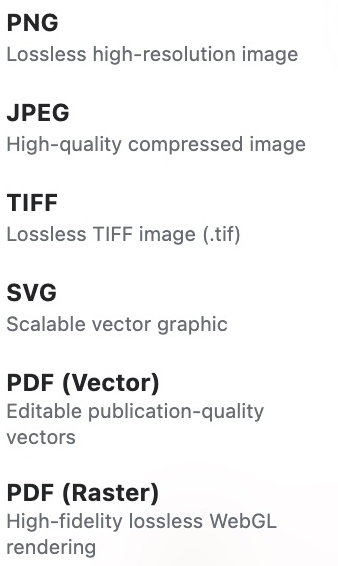
\includegraphics[width=52mm]{publication-assets/crop-496bc1fbfb3e99bfc4e7.png}
\end{minipage}\hspace{4mm}%
\begin{minipage}[t]{58mm}
\vspace{0pt}
{\centering
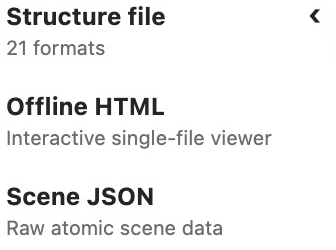
\includegraphics[width=51mm]{publication-assets/crop-68b4df9ea7d48ce9da1e.png}\par}
\par\vspace{3mm}
\raggedright\fontsize{9}{13}\selectfont
\ui{Structure file} saves the model information supported by the selected format.

\smallskip
\ui{Offline HTML} provides an interactive view in a local browser.

\smallskip
\ui{Scene JSON} records the atomic scene and is distinct from structure JSON.
\end{minipage}
\caption{The atomic viewer's export menus. \ui{Export image} on the left offers six image formats. \ui{Export file} on the right provides structure files, an offline page, and scene JSON.}
\label{fig:atomic-export-menus}
\end{figure}


\subsection{Save an interactive offline page}
\index{Offline HTML}

\ui{Offline HTML} bundles the current atomic scene, viewer appearance, and camera into one HTML file. It is useful for supplying a rotatable structure with a report. It supports viewing but does not replace a project containing workflows, calculation data, and editing history.

\begin{steps}
\item Choose the representation, repetitions, and initial view in the atomic viewer.
\item Choose \ui{Export file → Offline HTML} and save or download the \file{-offline.html} file.
\item Open it in a local browser. Check the initial structure and appearance, drag to rotate, scroll to zoom, and inspect the required atom information.
\item Identify the structure and purpose when sharing it. Include native structures and projects as well if the recipient needs to continue modeling or calculating.
\end{steps}

The offline page retains the scene at export. To reanalyze bonds, convert cells, or commit further model changes in the toolbox, return to the project and export a new page afterward.

\subsection{Distinguish scene \headinglatin{JSON} from structure \headinglatin{JSON}}

\ui{Scene JSON} in \ui{Export file} records atomic scene data, including sites, displayed images, connections, and analysis descriptions. It does not save the current camera and all appearance settings as a viewer configuration, and does not replace a project or calculation input.

For continued editing, choose native JSON under \ui{Structure file}. Reimporting it exposes the lattice, sites, periodicity, and properties; \file{properties} can retain twist angles, SQS search records, and other metadata. Files named \file{-scene.json} record scenes, while \ui{Offline HTML} supports offline viewing. Name files by purpose to distinguish them.

The supplied \file{ethanol-angle1095.json} describes the neutral singlet ethanol used here: 9 atoms, 8 explicit bonds, and a $109.5^\circ$ angle defined by 1(C)—2(C)—3(O). \mbox{\file{ethanol-angle1095.png}} is a 4032\,$\times$\,1964-pixel PNG exported from the same model; \file{ethanol-angle1095-scene.json} records the atomic scene. Import the structure JSON for editing; use the other two for illustration and scene inspection.

\subsection{Create a \headinglatin{Hero Shot}}
\index{Hero Shot}

Hero Shot presents the atomic scene with an emphasis on overall form and depth. Progressive rendering refines a PNG; its lighting and materials do not change atomic positions or electronic structure results.

\begin{steps}
\item Under \ui{Style → Theme}, select \ui{Gleamoe Noir}.
\item Find \ui{Hero Shot} and click \ui{Enter Hero mode}. Settings collapse and a dedicated framing interface opens.
\item Rotate and zoom the structure, using crystal-axis buttons if helpful. Hold the view still once composed so that progressive rendering can refine it.
\item Open \ui{Export Hero Shot} and start with \ui{High}. \ui{High}, \ui{Ultra}, and \ui{Poster} specify export scales of 2.5, 3, and 4 times the viewport.
\item Choose a location and wait for rendering and writing. Open \file{-hero.png} to check framing and detail; in Online, also confirm the browser download.
\item Click \ui{Exit Hero mode} to return to measurement or editing. Save the project and native model through their usual procedures.
\end{steps}

Start with a small model and High quality to compare framing and rendering easily. Conventional structure figures suit clear annotations and geometric comparisons; Hero Shot emphasizes form. Scientific descriptions still need model provenance, periodicity, and relevant dimensions.

\section{Export calculation figures}

\subsection{Choose a suitable format}

Figure documents provide axes tools for zooming, panning, and image export. Before exporting, check that labels and units are complete and lines are not clipped. Screenshots document interface operations; direct exports generally suit research data figures better.

Raster formats such as PNG work well in documents and presentations. PDF and SVG can retain crisp lines and text, although complex figures or certain rendering elements may use different output methods. Open the export to check text, lines, and rendering.

Online exports through the browser. Check the browser's actual download location rather than a server-side session path. Desktop editions use the location selected in the file dialog.

\subsection{Inspect details interactively}

Move over the axes and use the tools available for the current figure to pan, zoom, rotate, or restore the view. Enlarge the last few SCF iterations in a 2D convergence plot; rotate Brillouin zones or band surfaces. Restore the full range before exporting a complete result, rather than inadvertently saving a magnified fragment.

Three-dimensional band surfaces mainly show two band-edge surfaces. Their separation is not automatically the global gap: another direction may contain a lower conduction minimum or higher valence maximum. A Brillouin-zone plot shows reciprocal-space geometry, not energies encoded by polyhedron color. Band surfaces, zones, path bands, and DOS represent different quantities; identify the figure type in its caption.

\subsection{Export a figure from Online}

Online retains native figure toolbars, but save and copy actions obtain files through the browser. Saving an image opens an export dialog with filename, format, and resolution. Project saving and image download are separate operations.

\begin{steps}
\item Open the result and restore the desired axes range.
\item Choose save from the figure toolbar and enter a descriptive name, such as \file{H2-SCF.png}.
\item Choose PNG, JPEG, TIFF, PDF, or SVG. Raster resolution can range from 72 to 600 DPI. Start with 150 DPI for screen reading and increase it for print.
\item Click \ui{Save} and complete the browser download.
\item Open the downloaded file locally and check the axes, legend, and values needed for the caption.
\end{steps}

Copy-image and copy-vector actions also become file-retrieval workflows in a browser. Vector copying supplies SVG content rather than guaranteeing transfer to the operating system clipboard. For PDF and SVG, a DPI setting does not replace checking fonts, lines, and actual output. An image does not retain all original arrays; keep the project and required data too.

\subsection{Retain the numerical data}
\index{Data export}

Projects retain run data, and accompanying scripts provide MAT or CSV results for further calculation and consistently styled plots. Give CSV columns clear meanings, such as energy relative to the Fermi level followed by DOS. A separate units note is more reliable than a verbal explanation.

Use original numerical records for fitting, integration, or quantitative comparisons. Screenshots show trends, but values read from them depend on axes limits, resolution, and line width.

\subsection{Make figures understandable on their own}

A caption should explain the figure without requiring the reader to inspect the entire project. For a structure, identify atoms and the cell; for convergence, the iterated quantities and units; for bands, the path and energy zero; for DOS, the sampling and energy reference. Put key conditions in the caption or nearby text rather than crowding a complete log into the image.

Use consistent fonts, sizes, colors, and energy ranges. Reuse a color for the same quantity across figures. Show initial and optimized hydrogen structures from the same angle, or give two DOS plots matching limits. Such choices aid comparison more than decoration.

\section{Write a complete account of the result}

A clear description states the question, conditions, observations, and interpretation. For example, begin with optimizing the hydrogen bond length in a fixed $10$ Bohr box, specify PBE, pseudopotentials, and cutoff, report the shorter bond and lower energy, then explain that these describe equilibrium within the chosen model.

Avoid only saying that a result is normal or as expected. State which quantity converged, where the main change occurred, and which conditions were held fixed. Explain numerical accuracy in terms of the cutoff, sampling, and stopping criteria.

Before closing the project, save it and check that the project, inputs, and exported figures correspond. A project that can be reopened, interpreted, and run again is the fullest record of the calculation.
